\documentclass[aspectratio=169,11pt]{beamer}

% ============================================================
% THEME & COLOURS (matched to GDP PowerPoint)
% ============================================================
\usetheme{default}
\usecolortheme{default}
\setbeamertemplate{navigation symbols}{}

\definecolor{gdpPurple}{HTML}{633E88}
\definecolor{gdpDarkBlue}{HTML}{0C406D}
\definecolor{gdpNavy}{HTML}{091932}
\definecolor{gdpOrange}{HTML}{DD7A0F}
\definecolor{gdpSlate}{HTML}{3B4950}
\definecolor{gdpLightGray}{HTML}{E7E6E6}
\definecolor{gdpBurgundy}{HTML}{820E21}

\setbeamercolor{background canvas}{bg=white}
\setbeamercolor{normal text}{fg=gdpSlate}
\setbeamercolor{frametitle}{fg=gdpPurple,bg=white}
\setbeamercolor{framesubtitle}{fg=gdpDarkBlue,bg=white}
\setbeamercolor{title}{fg=gdpPurple}
\setbeamercolor{subtitle}{fg=gdpDarkBlue}
\setbeamercolor{author}{fg=gdpSlate}
\setbeamercolor{institute}{fg=gdpSlate}
\setbeamercolor{date}{fg=gdpSlate}
\setbeamercolor{item}{fg=gdpDarkBlue}
\setbeamercolor{subitem}{fg=gdpPurple}
\setbeamercolor{block title}{fg=white,bg=gdpDarkBlue}
\setbeamercolor{block body}{fg=gdpSlate,bg=gdpLightGray!30}
\setbeamercolor{block title alerted}{fg=white,bg=gdpBurgundy}
\setbeamercolor{block body alerted}{fg=gdpSlate,bg=gdpLightGray!30}
\setbeamercolor{footline}{fg=gdpSlate}

\usepackage{helvet}
\renewcommand{\familydefault}{\sfdefault}
\usepackage{amsmath,amssymb,graphicx,booktabs,array}
\usepackage{pifont}
\newcommand{\cmark}{\ding{51}}
\newcommand{\xmark}{\ding{55}}

\setlength{\tabcolsep}{3pt}
\setbeamertemplate{itemize/enumerate body begin}{\small}
\setbeamertemplate{itemize/enumerate subbody begin}{\footnotesize}
\addtolength{\leftmargini}{-0.3cm}
\addtolength{\leftmarginii}{-0.2cm}

\setbeamertemplate{frametitle}{%
  \vspace{0.2cm}
  \textbf{\large\insertframetitle}
  \vspace{0.05cm}
  \par\textcolor{gdpDarkBlue}{\rule{\textwidth}{1.2pt}}
  \vspace{-0.3cm}
}

\setbeamertemplate{footline}{%
  \leavevmode%
  \hbox{%
    \begin{beamercolorbox}[wd=.333\paperwidth,ht=2.5ex,dp=1ex,leftskip=0.3cm]{footline}%
      \insertshortauthor
    \end{beamercolorbox}%
    \begin{beamercolorbox}[wd=.333\paperwidth,ht=2.5ex,dp=1ex,center]{footline}%
      \insertshorttitle
    \end{beamercolorbox}%
    \begin{beamercolorbox}[wd=.333\paperwidth,ht=2.5ex,dp=1ex,rightskip=0.3cm]{footline}%
      \insertframenumber{}
    \end{beamercolorbox}%
  }%
}

\setbeamertemplate{title page}{
  \vspace{1.5cm}
  \begin{center}
    {\Huge\bfseries\textcolor{gdpPurple}{\inserttitle}}\\[0.4cm]
    {\Large\textcolor{gdpDarkBlue}{\insertsubtitle}}\\[1.2cm]
    {\large\textcolor{gdpSlate}{\insertauthor}}\\[0.3cm]
    {\normalsize\textcolor{gdpSlate}{\insertinstitute}}\\[0.3cm]
    {\normalsize\textcolor{gdpSlate}{\insertdate}}
  \end{center}
}

\title{Acoustic Wave Logic in a Y-Junction}
\subtitle{From Theory to FDTD Simulation}
\author{MSc Individual Research Project}
\institute{Cranfield University\hspace{0.3cm}|\hspace{0.3cm}Supervisors: Prof. Weisi Guo, Prof. Takis Tsoutsanis}
\date{\today}

\begin{document}

% ============================================================
\begin{frame}[plain]
  \titlepage
\end{frame}

% ============================================================
\begin{frame}{The Literature Landscape}
  \textbf{Every area we searched contributes a piece, but no one combines them all:}
  \vspace{0.15cm}

  \begin{table}
    \centering
    \footnotesize
    \renewcommand{\arraystretch}{1.05}
    \begin{tabular}{@{}lcccc@{}}
      \toprule
      & \textbf{Porous} & \textbf{Fluid} & \textbf{Parallel} & \textbf{Trainable} \\
      \midrule
      Porous memristors & \cmark & \cmark\ (ions) & \xmark & \xmark \\
      Bubble logic & \xmark & \cmark & \cmark & \xmark \\
      Chemical NNs & \xmark & \cmark & \xmark & \cmark \\
      Acoustic metasurfaces & \xmark & \xmark & \xmark & \xmark \\
      Diffractive optical NNs & \xmark & \xmark & \cmark & \cmark \\
      \midrule
      \textbf{Porous wave computing?} & \textbf{\cmark} & \textbf{?} & \textbf{\cmark} & \textbf{\cmark} \\
      \bottomrule
    \end{tabular}
  \end{table}

  \vspace{0.1cm}
  {\small \textbf{The gap:} A trainable, 3D, porous substrate for acoustic wave computation. No one has done it.}
\end{frame}

% ============================================================
\begin{frame}{Background: Hughes et al. (2019)}
  \textbf{Wave Physics as an Analog Recurrent Neural Network} — \textit{Science Advances} 5(12), eaay6946.

  \vspace{0.2cm}
  \begin{columns}[T]
    \begin{column}{0.55\textwidth}
      \footnotesize
      \textbf{What they found:}
      \begin{itemize}
        \item Wave equation in an inhomogeneous medium $\equiv$ RNN update rule.
        \item Material properties (wave speed, density) act as ``weights.''
        \item Demonstrated \textbf{vowel classification} on raw audio signals.
      \end{itemize}
    \end{column}
    \begin{column}{0.43\textwidth}
      \footnotesize
      \textbf{Why it matters:}
      \begin{itemize}
        \item Structured acoustic media as trainable computation substrates.
        \item Maps to porous media: porosity sets local wave speed.
      \end{itemize}
    \end{column}
  \end{columns}
\end{frame}

% ============================================================
\begin{frame}{Background: Lin et al. (2018)}
  \textbf{All-Optical Machine Learning Using Diffractive Deep Neural Networks} — \textit{Science} 361(6406), 1004–1008.

  \vspace{0.2cm}
  \begin{columns}[T]
    \begin{column}{0.55\textwidth}
      \footnotesize
      \textbf{What they found:}
      \begin{itemize}
        \item Built a \textbf{diffractive deep neural network} (D$^2$NN) using cascaded diffractive optical elements (DOEs) 3D-printed as phase-modulating layers.
        \item Each DOE acts as a layer of artificial neurons; pixel-wise phase delays represent weights.
        \item The system classifies images of \textbf{handwritten digits at the speed of light}.
      \end{itemize}
    \end{column}
    \begin{column}{0.43\textwidth}
      \footnotesize
      \textbf{Why it matters for us:}
      \begin{itemize}
        \item Layered scattering architecture $\rightarrow$ our inspiration for multi-layer acoustic diffractive slices.
        \item Proves that \textbf{wave interference alone} can implement neural-network-style computation without digital electronics.
      \end{itemize}
    \end{column}
  \end{columns}
\end{frame}

% ============================================================
\begin{frame}{Background: Wang et al. (2019)}
  \textbf{Binary-Phase Acoustic Passive Logic Gates} — \textit{Scientific Reports} 9, 8355.

  \vspace{0.15cm}
  \footnotesize
  \begin{columns}[T]
    \begin{column}{0.52\textwidth}
      \textbf{What they found:}
      \begin{itemize}
        \item Tri-port waveguide (two inputs A \& B, one output O) implementing Boolean logic via phase-controlled acoustic interference.
        \item Logic demonstrated: OR, NOT, AND, XOR (basic); XNOR, NOR, NAND, A$\odot$(B+C) (composite).
        \item Uses binary-phase passive unit cells (Helmholtz resonator arrays) to manipulate phase without active components.
      \end{itemize}
    \end{column}
    \begin{column}{0.46\textwidth}
      \textbf{Key design numbers:}
      \begin{itemize}
        \item Medium: Air ($c = 343$ m/s) in epoxy resin waveguide
        \item Operating frequency: \textbf{3.43 kHz}
        \item Wavelength: \textbf{100 mm} (in air)
        \item Gate dimensions: \textbf{0.6$\lambda$ length $\times$ 0.3$\lambda$ width}
        \item Fractional bandwidth: \textbf{~0.2}
        \item Logic threshold: \textbf{0.4 Pa} (input amplitude 1.0 Pa)
      \end{itemize}
    \end{column}
  \end{columns}

\end{frame}

% ============================================================
\begin{frame}{The Governing Equation}
  We solve the \textbf{2D scalar acoustic wave equation} in a homogeneous medium:
  \[
    \nabla^2 p(\mathbf{r},t) - \frac{1}{c^2}\frac{\partial^2 p}{\partial t^2} = 0
  \]
  where $p$ is acoustic pressure, $c$ is wave speed, and $\mathbf{r} = (x,y)$.

  \vspace{0.3cm}
  \textbf{Boundary conditions in our FDTD implementation:}
  \begin{itemize}
    \item \textbf{Rigid walls (Neumann):} $\partial p/\partial n = 0$ — implemented via ghost-cell reflection in the 5-point Laplacian stencil.
    \item \textbf{Hard source:} Sinusoidal pressure overwrite at inlet boundaries (no accumulation).
    \item \textbf{Open boundaries:} Zero-gradient (Neumann) at domain edges.
  \end{itemize}

  \vspace{0.2cm}
  \textcolor{gdpSlate}{\small We use second-order central differences in space and time (leapfrog) with a boundary-mask array for geometric flexibility.}
\end{frame}

% ============================================================
\begin{frame}{Our Simulation: Setup and Parameters}
  Design scaled from Wang's $0.3\lambda$ rule to microfluidic-relevant dimensions in water.

  \vspace{0.15cm}
  \begin{columns}[T]
    \begin{column}{0.48\textwidth}
      \footnotesize
      \textbf{Physical constants}
      \begin{itemize}
        \item Medium: water, $c = 1500$ m/s
        \item Frequency $f = 1$ MHz $\rightarrow$ $\lambda = 1.5$ mm
        \item Grid spacing $\Delta x = 50$ $\mu$m (30 cells/$\lambda$)
        \item CFL = 0.5 $\rightarrow$ $\Delta t \approx 11.8$ ns
      \end{itemize}
    \end{column}
    \begin{column}{0.48\textwidth}
      \footnotesize
      \textbf{Domain and geometry}
      \begin{itemize}
        \item Domain: $250 \times 200$ cells (12.5 mm $\times$ 10 mm)
        \item Inlet channels: 83 cells ($\approx$4.2 mm, 2.8$\lambda$)
        \item Merge angle: 60$^\circ$ total ($\pm$30$^\circ$)
        \item Channel width: 9 cells (0.45 mm, \textbf{0.3$\lambda$})
        \item Outlet probe: 60 cells downstream of merge
      \end{itemize}
    \end{column}
  \end{columns}

  \vspace{0.2cm}
  \footnotesize
  \textcolor{gdpBurgundy}{\textbf{Caveat:} Idealised values. Real devices exhibit temperature-dependent $c$, viscous losses, and 3D effects not captured here.}
\end{frame}

% ============================================================
\begin{frame}{Step 1: Solver Validation}
  Before adding geometry, we verify that the bare 2D solver reproduces expected physics.

  \begin{columns}[T]
    \begin{column}{0.48\textwidth}
      \footnotesize
      \textbf{Checks performed:}
      \begin{itemize}
        \item Point source produces circular wavefronts
        \item Amplitude decays as $1/\sqrt{r}$ in 2D
        \item Measured wavelength matches $\lambda = c/f$
      \end{itemize}
      \textbf{Result:} All checks passed. $1/\sqrt{r}$ decay confirmed by log-log fit.
    \end{column}
    \begin{column}{0.48\textwidth}
      \centering
      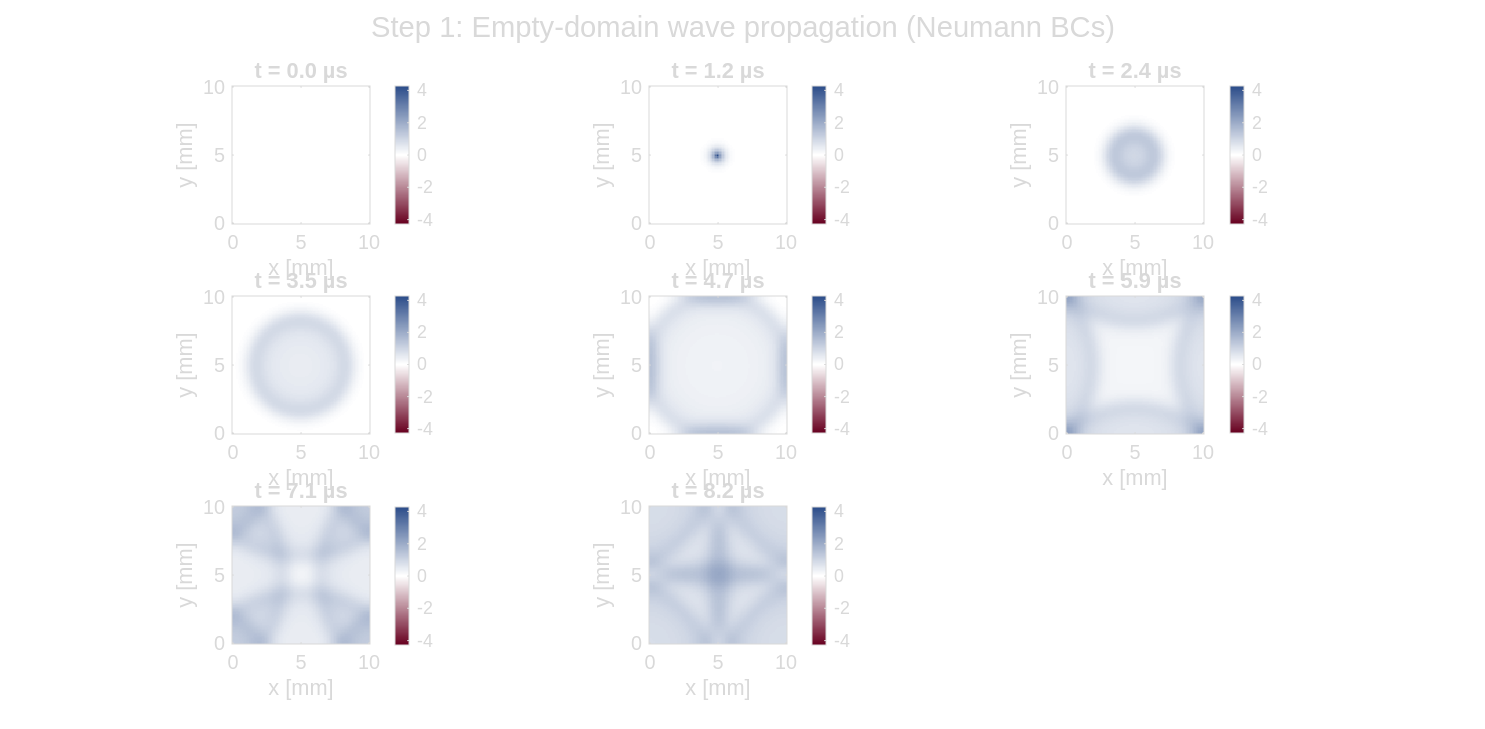
\includegraphics[width=0.85\textwidth]{../Analysis/y_junction_fdtd/figures/step1_empty_domain.png}
      \footnotesize Circular wavefronts from point source
    \end{column}
  \end{columns}

  \vspace{0.1cm}
  \textcolor{gdpSlate}{\small Confirms core leapfrog update and 5-point Laplacian stencil are correct.}
\end{frame}

% ============================================================
\begin{frame}{Step 2: Y-Junction Geometry and Steady-State Field}
  \begin{columns}[T]
    \begin{column}{0.48\textwidth}
      \centering
      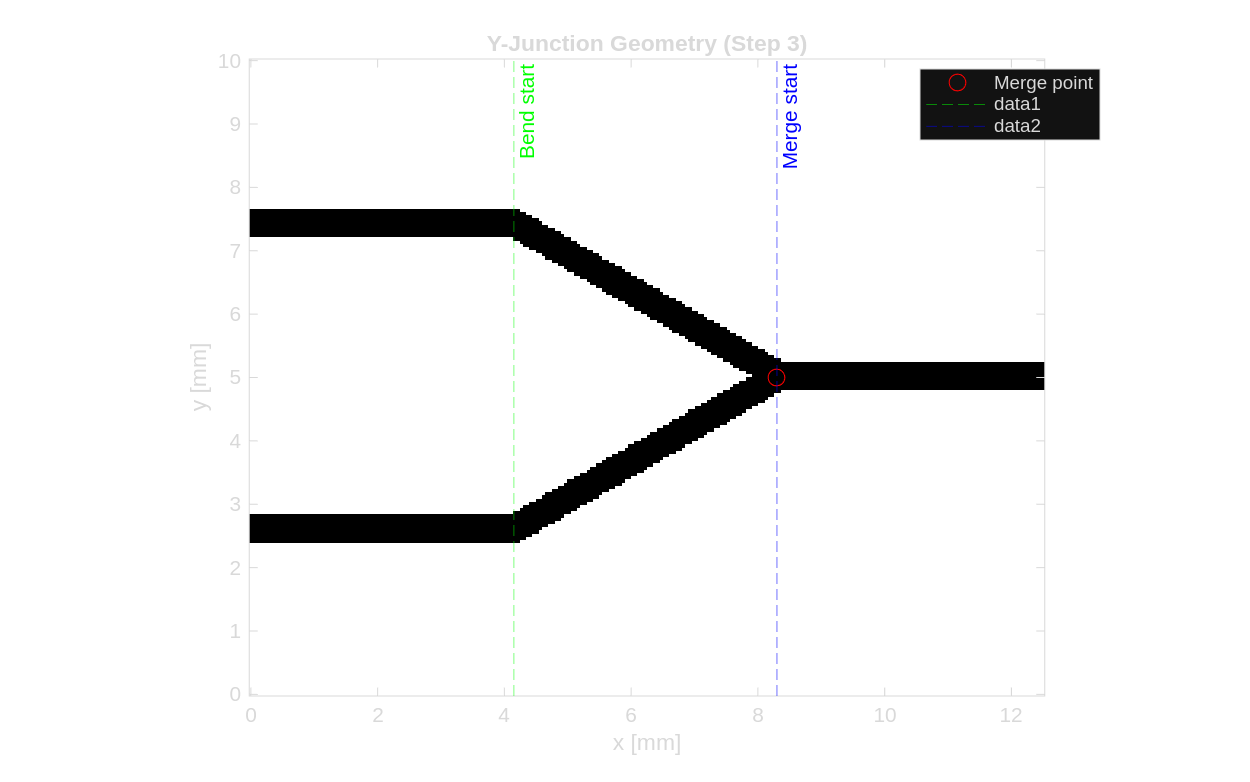
\includegraphics[width=0.70\textwidth]{../Analysis/y_junction_fdtd/figures/step3_geometry.png}
      \footnotesize Geometry mask (white = wall)
    \end{column}
    \begin{column}{0.48\textwidth}
      \centering
      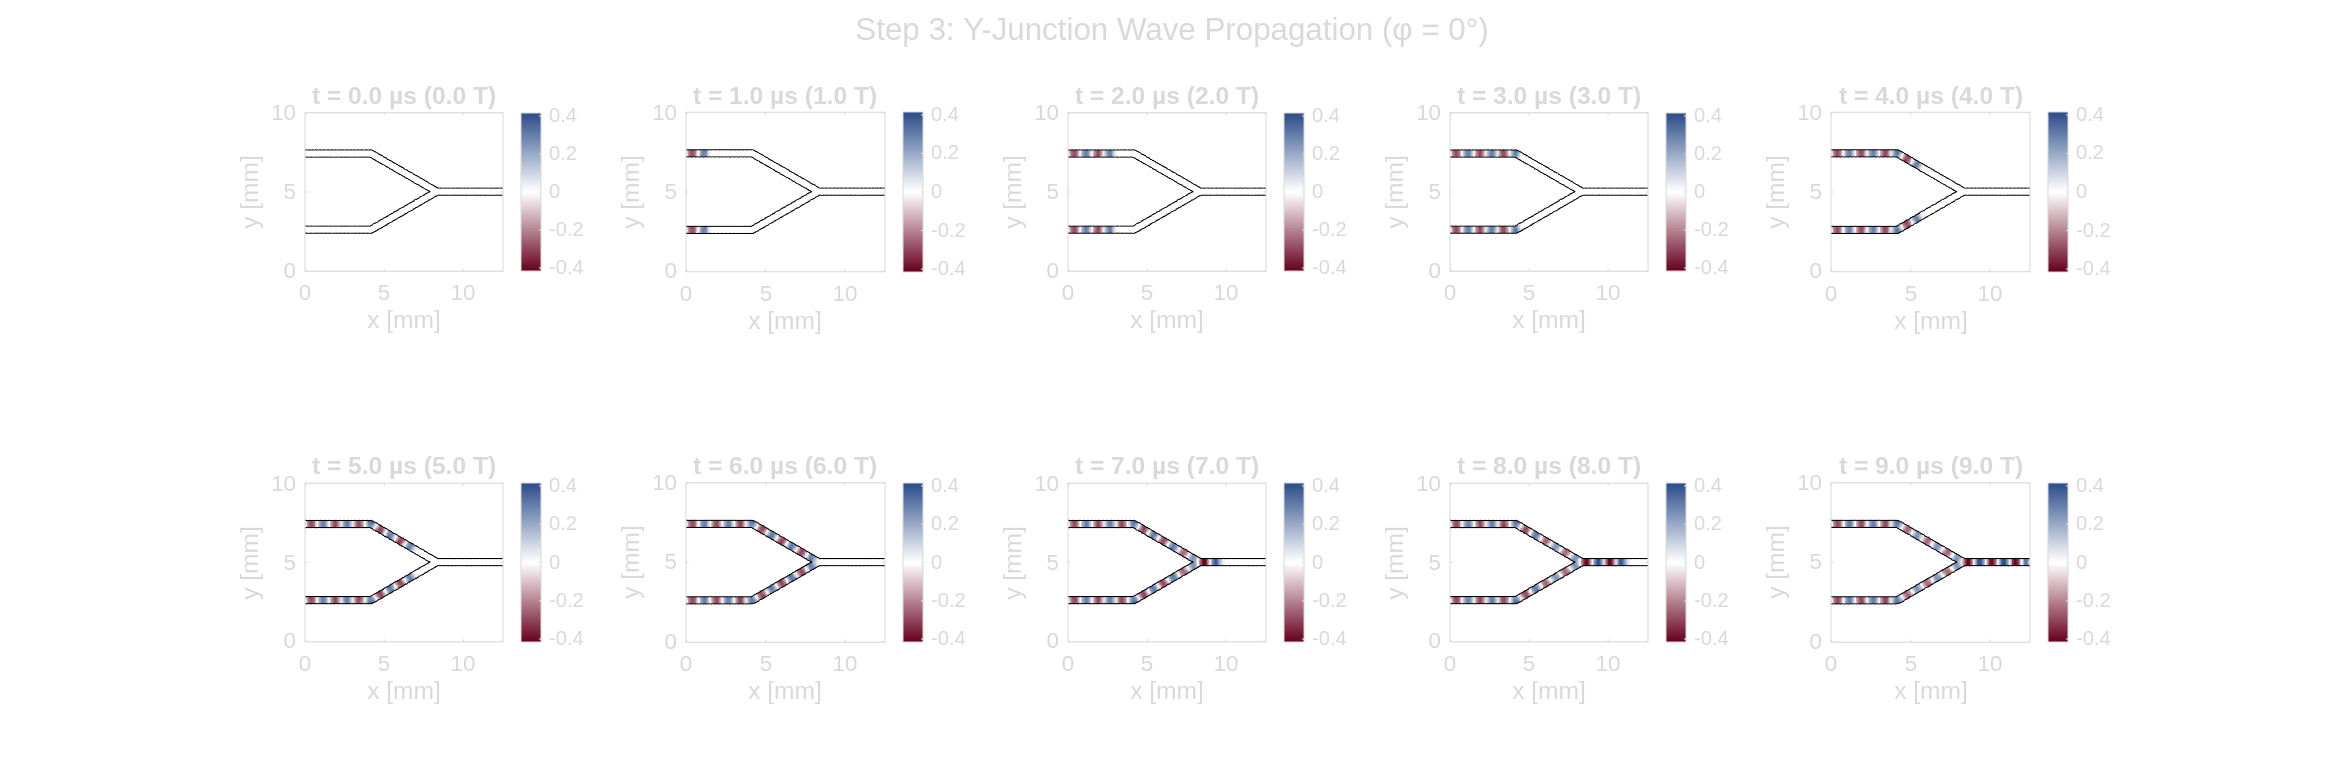
\includegraphics[width=0.70\textwidth]{../Analysis/y_junction_fdtd/figures/step3_y_junction.png}
      \footnotesize Pressure field at steady state ($\phi = 0^\circ$)
    \end{column}
  \end{columns}

  \vspace{-0.1cm}
  \footnotesize
  \textbf{Implementation choices:}
  \begin{enumerate}
    \item \textbf{Ghost-cell reflection:} Neumann BCs at internal boundaries without staircasing.
    \item \textbf{Frozen walls:} Wall cells reset after each step, preventing ``ringing.''
  \end{enumerate}
\end{frame}

% ============================================================
\begin{frame}{Step 3: Phase-Sweep Logic Demonstration}
  13 simulations, phase difference $\phi$ from $0^\circ$ to $360^\circ$ in $30^\circ$ steps.

  \centering
  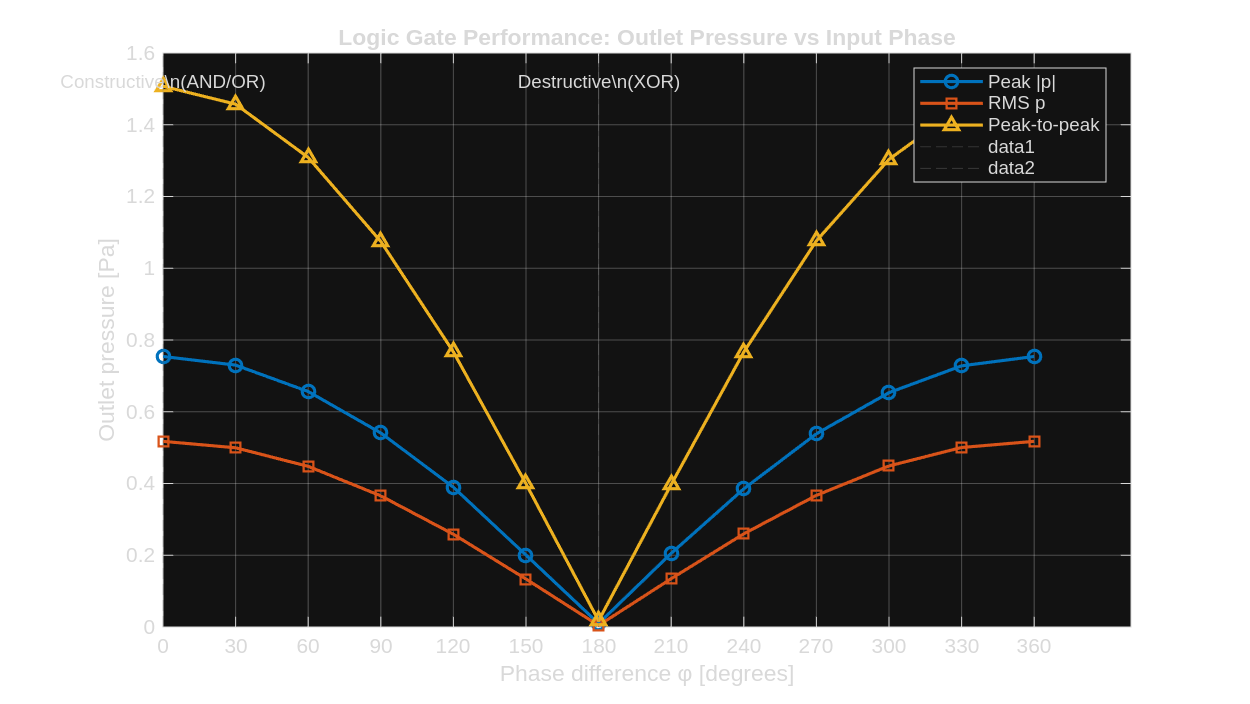
\includegraphics[width=0.52\textwidth]{../Analysis/y_junction_fdtd/figures/step4_phase_sweep.png}

  \vspace{0.05cm}
  \footnotesize
  \textbf{Behaviour matches interference theory:}
  \begin{itemize}
    \item Maximum at $\phi = 0^\circ$ (constructive)
    \item Minimum at $\phi = 180^\circ$ (destructive)
    \item Cosine-squared modulation
  \end{itemize}
\end{frame}

% ============================================================
\begin{frame}{Step 3: Field Snapshots and Logic Contrast}
  \begin{columns}[T]
    \begin{column}{0.52\textwidth}
      \centering
      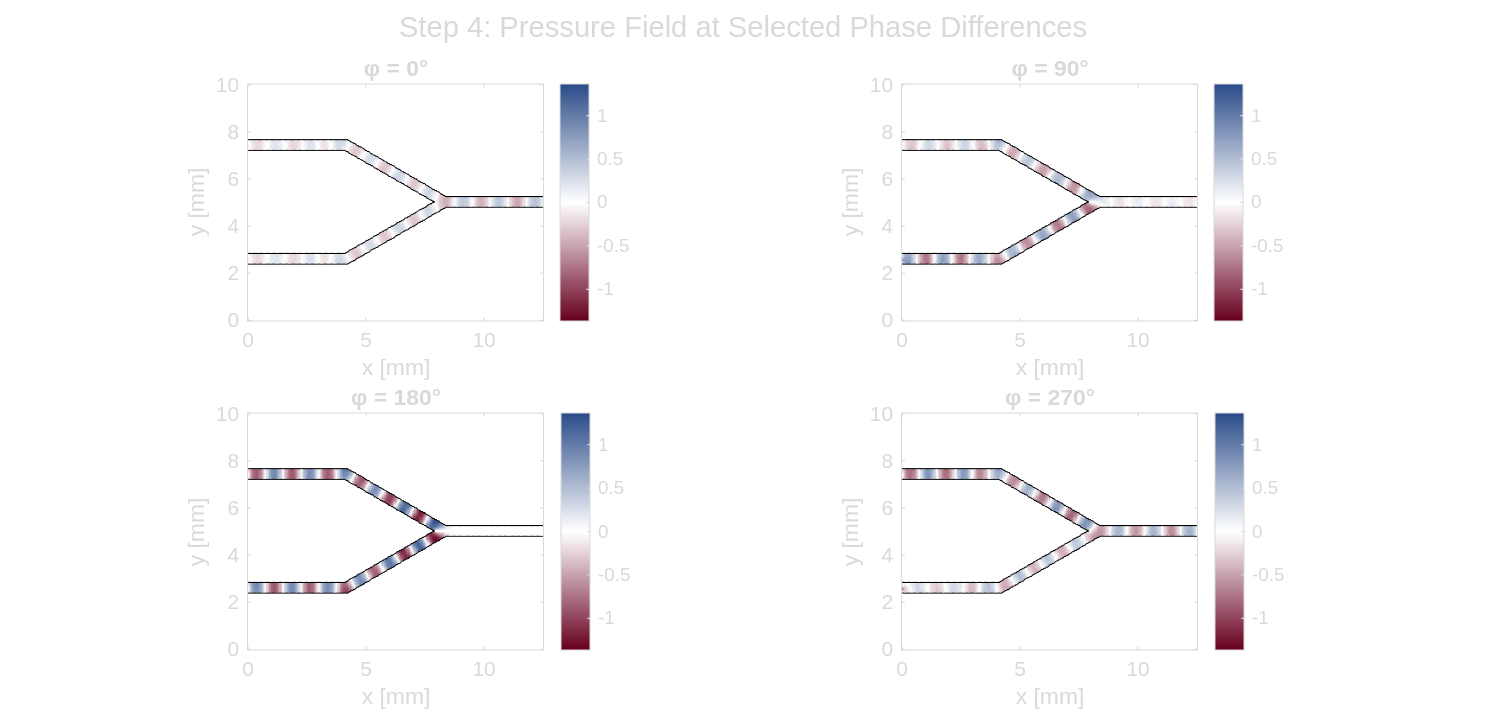
\includegraphics[width=0.65\textwidth]{../Analysis/y_junction_fdtd/figures/step4_snapshots.png}
      \footnotesize Pressure fields at $\phi = 0^\circ$, $90^\circ$, $180^\circ$, $270^\circ$
    \end{column}
    \begin{column}{0.46\textwidth}
      \centering
      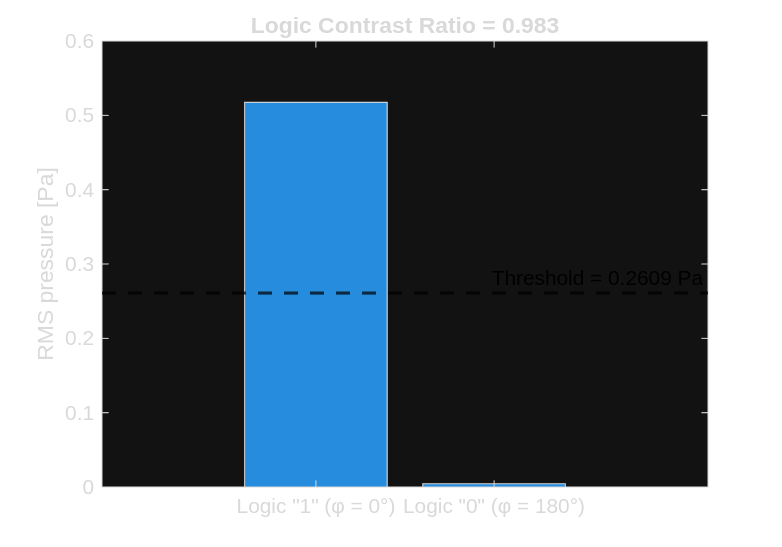
\includegraphics[width=0.63\textwidth]{../Analysis/y_junction_fdtd/figures/step4_logic_contrast.png}
      \footnotesize Logic contrast bar chart
    \end{column}
  \end{columns}

  \vspace{-0.1cm}
  \footnotesize
  \textbf{What the fields show:}
  \begin{itemize}
    \item At $\phi = 0^\circ$: waves align; maximum pressure exits
    \item At $\phi = 180^\circ$: merge is a node; outlet is near-silent
    \item Bar chart confirms clean HIGH/LOW separation
  \end{itemize}
\end{frame}

% ============================================================
\begin{frame}{Step 3: The Numbers}
  RMS pressure measured at the outlet probe over the last 3 periods (after transient decay).

  \vspace{0.15cm}
  \begin{columns}[T]
    \begin{column}{0.55\textwidth}
      \centering
      \footnotesize
      \renewcommand{\arraystretch}{1.05}
      \begin{tabular}{@{}lcc@{}}
        \toprule
        \textbf{Phase $\phi$} & \textbf{Peak $|p|$ (Pa)} & \textbf{RMS (Pa)} \\
        \midrule
        $0^\circ$   & 0.840 & \textbf{0.573} \\
        $60^\circ$  & 0.701 & 0.495 \\
        $90^\circ$  & 0.564 & 0.399 \\
        $120^\circ$ & 0.419 & 0.288 \\
        $150^\circ$ & 0.220 & 0.149 \\
        $180^\circ$ & 0.000 & \textbf{0.000} \\
        \bottomrule
      \end{tabular}
    \end{column}
    \begin{column}{0.42\textwidth}
      \footnotesize
      \textbf{Key metrics:}
      \begin{itemize}
        \item Logic HIGH ($\phi = 0^\circ$): RMS = 0.573 Pa
        \item Logic LOW ($\phi = 180^\circ$): RMS = 0.000 Pa
        \item Contrast ratio: $\dfrac{0.573 - 0.000}{0.573 + 0.000} =$ \textbf{1.000}
        \item Threshold = 0.287 Pa
      \end{itemize}
    \end{column}
  \end{columns}

  \vspace{0.2cm}
  \textcolor{gdpBurgundy}{\small \textbf{Caveat:} Perfect null is idealised. Real devices have non-zero minimum from asymmetry, noise, viscosity, and 3D leakage.}
\end{frame}

% ============================================================
\begin{frame}{What This Demonstrates}
  \begin{enumerate}
    \item \textbf{Physical grounding:} A structured waveguide performs input-weighted interference exactly as predicted by linear acoustics.
    \item \textbf{Logic controllability:} Phase difference alone is sufficient to switch between HIGH and LOW states — no active valves or electronics inside the medium.
    \item \textbf{Scalable design rule:} Wang's $0.3\lambda$ width and $0.6\lambda$ length are dimensionless ratios that translate from air at 3.43 kHz to water at 1 MHz, confirming the geometry is media-agnostic.
    \item \textbf{Simulation fidelity:} The FDTD solver reproduces ideal interference patterns, giving confidence in the numerical framework for more complex geometries.
  \end{enumerate}

  \vspace{0.25cm}
  \textcolor{gdpDarkBlue}{\small This is a single ``neuron'' (one interference node). The next step is to cascade multiple such nodes into a trainable diffractive layer.}
\end{frame}

% ============================================================
\begin{frame}{Next Steps}
  \begin{columns}[T]
    \begin{column}{0.48\textwidth}
      \footnotesize
      \textbf{Short term (simulation):}
      \begin{itemize}
        \item \textbf{Diffractive slice:} Obstacle-array neural layer — a 2D acoustic adaptation of Lin et al.'s layered optical architecture.
        \item \textbf{Loss modelling:} Add viscous damping term to FDTD to estimate realistic contrast degradation.
        \item \textbf{Absorbing BCs:} Replace zero-gradient edges with PML to eliminate reflection artifacts.
      \end{itemize}
    \end{column}
    \begin{column}{0.48\textwidth}
      \footnotesize
      \textbf{Medium term (validation \& extension):}
      \begin{itemize}
        \item \textbf{OpenFOAM:} Validate reflection physics and pressure profiles against a finite-volume compressible solver.
        \item \textbf{Porous media:} Introduce stochastic pore networks and explore Biot's coupled wave modes as trainable parameters.
        \item \textbf{Thesis write-up:} Methodology chapter documenting FDTD framework, solver verification, and design rationale.
      \end{itemize}
    \end{column}
  \end{columns}

  \vspace{0.3cm}
  \begin{center}
    \Large\textbf{\textcolor{gdpPurple}{Questions / Discussion}}
  \end{center}
\end{frame}

\end{document}
